\section{Einleitung}

Worum gehts? Firewall Geschichte? Theorie und Technisches über iptables (extra Kapitel)
Die Einleitung \cite{iptables}

vpn server liegt auf fw2. client to lan erlauben. 1194 1195 müssen weitergeleitet werden. für welche dev müssen wir die vpn freigeben?

alles was von innen nach außen aufgebaut wird, soll erlaub werden.

route muss in srv1 ins fw2 netzwerk eingetragen werden

\subsection{Begriffsdefinitionen}

Masquarading? Hier oder im Konfig Kapitel?

Connection Tracking? Hier oder im Konfig Kapitel?

\paragraph{DMZ}
Wenn als Computernetzwerkbegriff verstanden ist die
\emph{demilitarisierte Zone} ein Bereich in dem Dienste einer Firma die nach Außen,
also z.B. das Internet oder Extranet, angeboten werden. Diese Dienste sollen
vom eigentelichen LAN in einem abgeschotteten Bereich laufen, so dass
beispielsweise die Mitarbeiterrechner sicher sind.


\section{Versuchsaufbau}

Ziel ist es das Firmen-LAN sowie die zugehörige DMZ durch die
{\tt iptables} Linux-Firewall abzusichern.

\begin{figure}[h!]
  \centering
    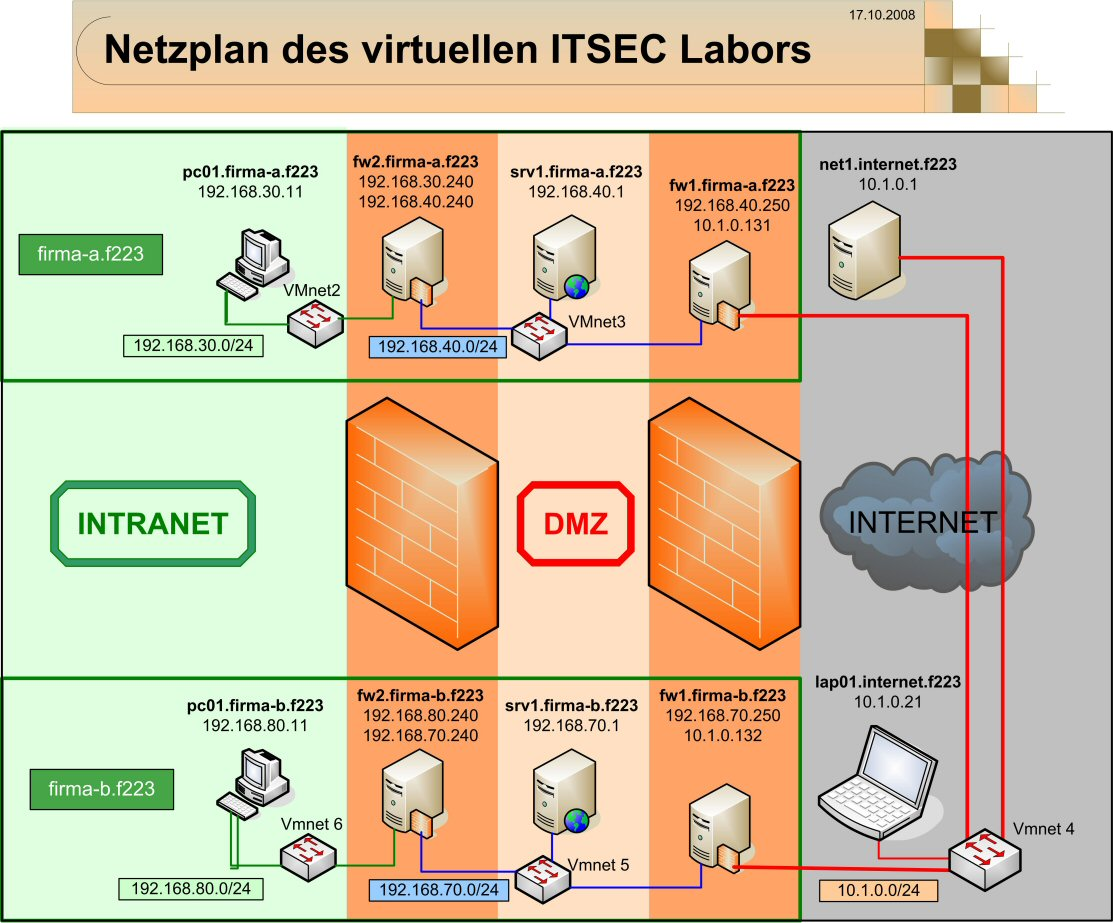
\includegraphics[width=0.9\textwidth]{figures/Netzplan.jpg}
  \caption{Netzplan des Versuchsaufbaus.\cite{labor}}
  \label{fig.netzplan}
\end{figure}

Dazu sind im Versuchsaufbau für jeden der in Abbildung 
\ref{fig.netzplan} abgebildeten Rechner
eine virtuelle Maschine bereitgestellt---dies ermöglicht leichteres
Testen.

Wir haben uns dazu entschieden, das Netzwerk der \emph{Firma A} aufzubauen.
Firma B bleibt unangetastet, und ist somit vollständig vorkonfiguriert,
was ein leichteres Testen ermöglicht.\cite{labor}


\section{Linux Konfiguration}

Zunächst müssen zwei Debian 6.0 Maschinen,
mit der minimalen Installation, eingerichtet werden.
Diese repräsentieren die Firewallmaschinen {\tt fw1} und {\tt fw2} aus
Abbildung \ref{fig.netzplan}.
Es wurde noch weitere Software installiert,
beschrieben in Kapitel \ref{sec.software}.
Die genaue Netzwerkadapterkonfiguration ist in Kapitel \ref{sec.netzwerk}

\subsection{Software}\label{sec.software}

Zusätzliche Software wurde via {\tt apt-get}, Debians Paketmanager,
installiert.

\begin{itemize}
    \item iptables
    \item iptstate---IPTables State Top.
    \item resolvconf---Nameserver information handler.
\end{itemize}


\subsection{Netzwerkadapter}\label{sec.netzwerk}

Die Netzweradapter wurden gemäß der in Abbildung \ref{fig.netzplan}
gezeigten IP-Adressen konfiguriert.
Die Konfigurationsdatei dazu liegt in {\tt /etc/network/interfaces}.

\subsubsection{\fwa}

Ist Firewall {\tt fw1} die zwischen \fwa sitzt.

\paragraph{eth0} Verbindung zur DMZ.

\begin{lstlisting}[label=lst:dmz:eth0,caption={Netzwerkadapter eth0 Konfiguration.}]
allow-hotplug eth0
iface eth0 inet static
    address 192.168.40.250
    netmask 255.255.255.0
    broadcast 192.168.40.255
    dns-nameservers 192.168.40.1
    dns-search firma-a.f223
\end{lstlisting}

\paragraph{eth1} Verbindung zum Extranet bzw. Internet.

\begin{lstlisting}[label=lst:extranet:eth1,caption={Netzwerkadapter eth1 Konfiguration.}]
allow-hotplug eth1
iface eth1 inet static
    address 10.1.0.131
    netmask 255.255.255.0
    broadcast 10.1.0.0
\end{lstlisting}


\subsubsection{\fwb}

Ist Firewall {\tt fw2} die zwischen \fwb sitzt.

\paragraph{eth0} Verbindung zum Intranet.

\begin{lstlisting}[label=lst:dmz:eth0,caption={Netzwerkadapter eth0 Konfiguration.}]
allow-hotplug eth0
iface eth0 inet static
    address 192.168.30.240
    netmask 255.255.255.0
    network 192.168.30.0
    broadcast 192.168.30.255
    dns-search firma-a.f223
\end{lstlisting}

\paragraph{eth1} Verbindung zur DMZ.

\begin{lstlisting}[label=lst:extranet:eth1,caption={Netzwerkadapter eth1 Konfiguration.}]
allow-hotplug eth1
iface eth1 inet static
    address 192.168.40.240
    netmask 255.255.255.0
    network 192.168.40.0
    broadcast 192.168.40.255
    dns-nameservers 192.168.40.1
\end{lstlisting}


\subsection{Nützliches}

\subsubsection{Einfacher Dateitransfer}

\noindent Empfänger:
\begin{verbatim}
fw2 $ netcat -l -p 8080 > firewall-internal.sh
\end{verbatim}

\noindent Sender:
\begin{verbatim}
fw1 $ cat firewall-external.sh | netcat 192.168.40.240 8080
\end{verbatim}


\subsection{Bootskript}

Debian verwendet das sogenannte \emph{Init Script LSB}\footnote{
\url{http://wiki.debian.org/LSBInitScripts}}, welches Unterstützung
für \emph{dependency based boot sequencing}\footnote{
\url{http://wiki.debian.org/LSBInitScripts/DependencyBasedBoot}
} bietet. Das bedeutet, dass
die Programme die beim Aufstarten des Betriebssystems in einer idealen
Reihenfolge angeordnet werden, so dass es auch keine unangenehme Effekte
durch Abhängigkeiten der Programme untereinander entstehen.

Diese Bootskripte werden in {\tt /etc/init.d/} als Konfigurationsdateien
abgelegt und beginnen mit wohldefinierten Kopfzeilen, wie in Listing
\ref{lst:lsb-header} gezeigt. In diesen Zeilen können die Abhängigkeiten
konfiguriert werden.

\begin{lstlisting}[label=lst:lsb-header,caption={Init Script LSB: Kopfzeilen.}]
### BEGIN INIT INFO
# Provides:          scriptname
# Required-Start:    $remote_fs $syslog
# Required-Stop:     $remote_fs $syslog
# Default-Start:     2 3 4 5
# Default-Stop:      0 1 6
# Short-Description: Start daemon at boot time
# Description:       Enable service provided by daemon.
### END INIT INFO
\end{lstlisting}

Wenn \emph{dependency-based booting} aktiviert ist, wird ein Daemon mit seinem
Startupskript aus {\tt /etc/init.d/} mit {\tt insserv}\footnote{
\emph{Vor} Debian 6.0 wird {\tt update-rc.d} verwendet.
} gestartet:

\begin{verbatim}
insserv mydaemon_script
\end{verbatim}

Nach den Kopfzeilen kommt das eigentliche Skript, welches z.B. mittels
{\tt iptables} die Firewall konfiguriert, aber auch beliebige andere Programme
und Dienste können somit gestartet werden.

\begin{lstlisting}[label=lst:lsb-script,caption={Init Script LSB: Eigentliches Skript.}]
case "$1" in
    start)
        # Startup stuff
        echo "Daemon started."
        ;;
    stop)
        # Shutdown this service
        echo "Daemon stopped."
        ;;
    restart)
        # Restart this service
        echo "Daemon restarted."
        ;;
    *)
        # The default case
        echo "Usage $0 {start|stop|restart}"
        ;;
esac
\end{lstlisting}


\section{Anforderungen}

\subsection{\fwa}

\paragraph{§ 1 Anforderungsname}

\subsection{\fwb}

